\chapter{Routing}

Even nowadays the routing is often done manually for analogue circuits. This is mainly caused by a lack of good tools and therefore the missing trust of engineers in them. The engineers consider a lot of different constraints during the routing, for example symmetries, net lengths and capacitive couplings. All these things have a major impact on the performance of the circuit, as in the analogue world it is very important to have a really accurate signal level, only high or low isn't enough.

The designer additonally adds guards and rings to the placement to protect certain devices from noise. This noise can come from for example the clock net or other routes, which carry a signal with high frequency. But high frequencies aren't the only disturbing effects, already during the placement the designer has to consider temperature gradients, caused by transistors with a high power consumption. To avoid problems with different temperatures in the substrate of for example the devices of differential pair the can be placed symmetric or can even have a common centroid. Around these grouped modules then the designer can create for example a guard ring around to protect the devices even more. An example for a manually routed layout can be seen in \nref{fig:miller_amplifier_routed_layout}.

So for an automatic routing algorithm a lot of different constraints must be considered. There are even more obstacles than just the devices and already created routes, for example the routes should pass over guard rings. To solve this problem in the following chapter are two different approaches presented: One simple sequentially line expansion router and one extend version of the previous one, which selects all routes together in one step. But first I have to discuss the changes that were necessary for the implementation of the routing algorithms.

\begin{figure}
	\centering
	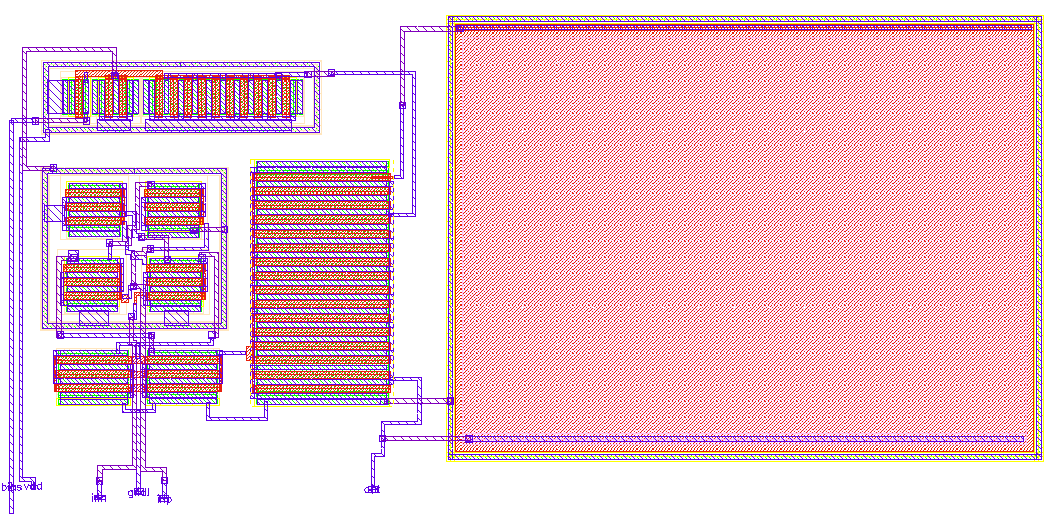
\includegraphics[scale=.4]{FIG/miller_amplifier_layout_routed.png}
  	\caption{manually routed layout of a miller amplifier}
	\label{fig:miller_amplifier_routed_layout}
\end{figure}

\section{Changes for Routing in the existing Applications}

\subsection{Plantage}

\subsubsection{Missing Data}
To actually route the placements some data was missing in plantage. Although at some points the routing was already prepared, example given the net names were available, but important information was not given. These include:
\begin{itemize}
\item Actual dimensions of the modules
\item Parameters for the technology
\item Vias and routes
\item Guard rings
\end{itemize}

In awareness of the necessary routing for every module a bigger area was defined for the placement. The additional space between the modules could then be used to route the placement. But the information about the actual dimension of the modules was missing.

The technology rules are passed through by the ICFBInterface to Plantage. At least for the technology definitions of Austria Microsystems it is not necessary to convert these rules, as the same format is chosen. For other manufacturers a conversion might be necessary.

The vias and routes were not considered at all previously. The main information which is needed to route are the dimension of the vias on the different layers and the width for the routes. Actually there is no real width for a route, but a minimal width, which a route must have. Usually this width is used for the routes. Also the dimensions for the via must be caculated, which can be done as described previously. Also the generated routes and placed vias needed to be added to the output of plantage, so that they can be shown in the GUI.

Previously every pin consisted only of one rectangle, which is obviously not enough. This basic information was used to minimize the estimated net length for the placements. But for real routing we need more complex possibilities to define pins, as, for example, the gate can be connected from both sides. Also it is not recommend to contact over the diffusion area. This will result in even more complex contact areas, as they could be split up in different parts. The definition of these areas is done by the user in the GUI and handed over to plantage. The used format defines for every pin, which a module has, at least one contact area, but eventually a lot more. During the routing then the acutal contact area is selected based on a certain heuristic.

\subsection{ICFBInterface}
The GUI-part of this application also needed some adaptions. This work was mainly done by Martin Keßler and contained the following parts:

\begin{itemize}
\item possibility to define contact areas
\item displaying routes and vias
\item possibility to change algorithm settings
\end{itemize}	

\section{Overview of Existing Routing Algorithms}

MISSING

\section{Implemented Routing Algorithms}
During this thesis two different routing algorithms were implemented: First of all a typical line expansion router. This solutions doesn't consider all constraints, but it is able to create at least reasonable results. Afterwards this algorithm was extended to consider additional constraints.

\subsection{Line Expansion Router}

\subsubsection{Select a Target}
The first thing which the algorithm has to do, before it can calculate a route, is to selected the start and target contact area. There can be several possibilities, as every pin can have several contact areas. Later on we will even see that already created routes can be candidates to start or end with a route. Basically this task can be seen as the selection of the closest rectangles of two lists of possibilities. For this I first want to talk a little bit about how the closest distance between two rectangles can be calculated.

For two rectangles there are several possible constellations. The first one we usually check is, if the overlap. If this is the case we can calculated easily the rectangle which is covered by both \nref{fig:rectangles_overlapping}. The distance is 0 in this case, and as start points for both rectangles we can select the center of gravity of the overlapping area.

\begin{figure}
	\centering
	\setlength{\unitlength}{0.282222229121mm}
\begin{picture}(275.80054, 174.07812)(0, -174.07812)
  \put(0,-174.07812){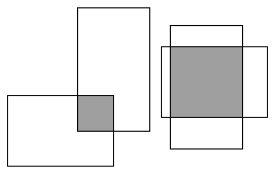
\includegraphics[height=49.1287150676mm, width=77.8370431916mm]{FIG/rectangles_overlapping.svg.pdf}}
\end{picture}
  	\caption{overlapping area of two rectangles is again a rectangle}
	\label{fig:rectangles_overlapping}
\end{figure}

If the two rectangles do not overlap it becomes a little bit more difficult. In this case we can at least say, that one of the rectangle has its closest point at one of the. Actually there can be even an endless count of solutions for this problem, but we are only interested in one of them. Because of this we select the easiest to calculate solution, which means the selection of a corner for one rectangle. The closest corner from the first rectangle to the second one is that one, which has the closest euclidean distance to the center of gravity of the second one \nref{fig:rectangles_closest_corner}. As we now know for one rectangle the closest point we can start to select the closest point on the second one. This point must be obviously on one of the edges. Every edges is basically a line segment, where the closest point can be calculated easily. For this task we first need the expansion of the line segment into a whole line. We then can turn this line 90 degrees (it doesn't matter in which direction as it is a line) and move this new line, so that it crosses our point, from which we want to know the closest point on the line segment. The crossing point of these two lines, if it is also inside the line segment, is the closest point. If this crossing point is outside the line segment the closest point must be the start or end point of the line segment, which are actually the rectangle's corners.

\begin{figure}
	\centering
	\setlength{\unitlength}{0.282222229121mm}
\begin{picture}(275.80054, 174.07812)(0, -174.07812)
  \put(0,-174.07812){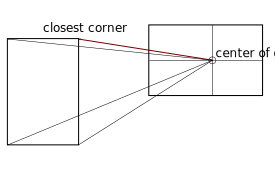
\includegraphics[height=49.1287150676mm, width=77.8370431916mm]{FIG/rectangles_closest_corner.svg.pdf}}
  \put(216.142843,-57.22096){\makebox(0,0)[l]{\smash{center of gravity}}}
  \put(43.019685,-31.84584){\makebox(0,0)[l]{\smash{closest corner}}}
\end{picture}
  	\caption{the closest corner is that one, which has the smallest distance to the center of gravity of the other one}
	\label{fig:rectangles_closest_corner}
\end{figure}

\subsubsection{Consider Obstacles}
After the algorithm has selected start and target contact areas the next step is to avoid routes across modules. For this purpose during all the following steps the modules are considered as obstacles. But during the first step usually the route has first to get out of the module. To avoid additional, accidentally added, gates the algorithm has to choose the shortest way to get out of the module. To decrease the resistance it is also possible to start right at the contact area to the next layer and use for example metal to get out of the module as fast as possible.

As the algorithm now has all the necessary information the actual line expansion routing can start. The main idea behind a line expansion router is that the routes are created sequentially. Every single step is based on a map of obstacles, which the route mustn't cross. From the starting point beginning always the next possible point of a route is calculated and the algorithm afterwards again applied to this partial problem. At the beginning of this recursive algorithm, as usual, the terminating condition is checked: If we have reached the target point. In every single step there are several decisions to be made: First the possible directions are grouped in good and bad directions \nref{fig:router_good_bad_direction}. Good directions are those, which reduce the distance to the target and bad ones are all the others.

\begin{figure}
	\centering
	\setlength{\unitlength}{0.282222229121mm}
\begin{picture}(322.55502, 271.89285)(0, -271.89285)
  \put(0,-271.89285){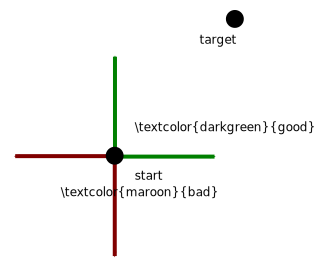
\includegraphics[height=76.7342062091mm, width=91.0321967586mm]{FIG/router_good_bad_direction.svg.pdf}}
  \put(134.88118,-180.46426){\makebox(0,0)[l]{\smash{start}}}
  \put(60.59547,-196.89285){\makebox(0,0)[l]{\smash{\textcolor{maroon}{bad}}}}
  \put(134.88118,-131.80496){\makebox(0,0)[l]{\smash{\textcolor{darkgreen}{good}}}}
  \put(199.88118,-43.8779){\makebox(0,0)[l]{\smash{target}}}
\end{picture}
  	\caption{good and bad directions}
	\label{fig:router_good_bad_direction}
\end{figure}

Additionally it makes no sense to go back the same direction where the last step came from. Also the same direction like the last step is not senseful. Because if this would be a good decision, the last step could have gone further. So these two directions are removed from the good directions. After this selection the router can make one step further in every good directon, as far as possible. This means, that the next step can go as far, as no obstacle is on the way or the target (in this coordinate) is reached \nref{fig:router_go_as_far_as_possible}.

\begin{figure}
	\centering
	\subfloat[no obstacle]{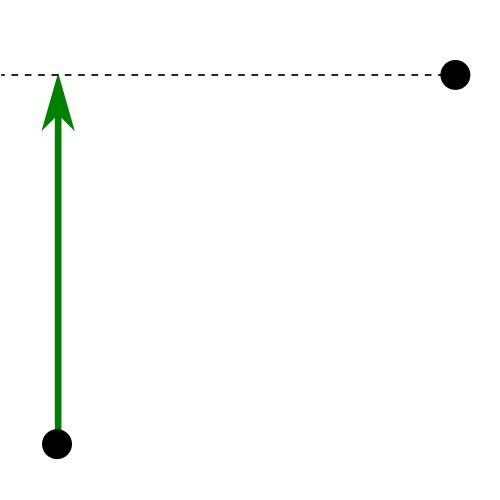
\includegraphics[scale=0.8]{FIG/router_as_far_as_possible.png}}
	\subfloat[with obstacle]{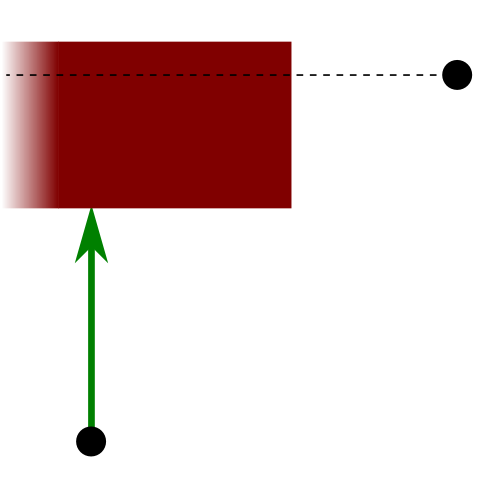
\includegraphics[scale=0.8]{FIG/router_as_far_as_possible_obstacle.png}}
	\caption{in a good direction the route can go as far as possible}
	\label{fig:router_go_as_far_as_possible}
\end{figure}


During the calculation of the steps towards the target I count those, which are feasible. If none of them is feasible the algorithm will have to select one of the bad directions for the next step. A major premission for this is also, that our last step ended at an obstacle. The router now can go as far as necessary into this bad direction \nref{fig:router_as_far_as_necessary}.

\begin{figure}
	\centering
	\setlength{\unitlength}{0.282222229121mm}
\begin{picture}(500.0, 300.0)(0, -300.0)
  \put(0,-300.0){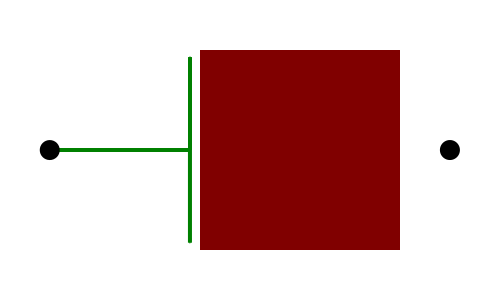
\includegraphics[height=84.6666687363mm, width=141.11111456mm]{FIG/router_as_far_as_necessary.svg.pdf}}
\end{picture}
 	\caption{a step into a bad direction should go only as far as necessary}
	\label{fig:router_as_far_as_necessary}
\end{figure}

Last but no least it is also possible to switch to the neighboured layers. For modules the obstacle can not be crossed with this way, as they are obstacles at every layer. But if for example the obstacle is just another route a layer switch may solve the problem.

\subsubsection{Avoid Collisions}
To avoid collisions I take in account the preferred directions for every layer. This information is again stored in the technology file and describes, if a layer should be used for horziontal or vertical routes. This reduces the possibility of collisions very efficiently and results in less complex layouts.

\subsubsection{Symmetric Routes}
In manually created layouts an usual way to route symmetric elements is to create them optical symmetric. This optical symmetry gives the designer an easy way to create symmetry. But the really important part about routing symmetries is to match the parasitics. The resistance of the route is for sure matched for the symmetric routes through an optical symmetry, but the capacitive couplings are obeyed in most cases. Therefore I have also concentrated on the resistance. To also consider the parasitics it would have been necessary to create all routes at the same time, because only with such an approach you can evaluate the capacitive parasitics, otherwise you never know what influence routes will have that will be created afterwards. As I have chosen to create the routes one by one I can't consider the capacities for the symmetries.

But before I go more into detail of the routing I want to explain the situation a bit more. Symmetries are caused by symmetry constraints, which can have, as already described earlier, single and pair modules. Single modules are quite useless for a symmetric routing. The only modules of interest are pair modules, no matter if they must be connected only together or also to another module.

In the routing first all modules are extracted, which are symmetric and where both parts of the symmetry pair must be connected to the same net. This pairs are then connected together and the only possible start or end point for other routes is than the middle of the route between the pair. In this case middle doesn't have to mean the same distance to both sides, but the same resistance to both modules. Therefore, if for example the route uses different layers from the modules to the middle, it is possible that the middle in terms of resistance doesn't have to be the same like the middle in terms of distance.

\subsubsection{Guard Rings}
With guards a designer can protect for example a certain signal from another very noisy one or protect whole module groups. The latter one is for example often used for current mirrors, as they are very sensitive against noise. In physical representation a guard or guard ring is only a layer, for example MET1, contacted to the substrate and connected to a certain Voltage level (often ground). For routing this results only in an additional obstacle on this layer.

PICTURE MISSING OF GUARD RING MET1

The major difference of guard rings to usual obstacles is, that they are obstacles only for certain nets. Or, if you look at it the other way round, a guard ring isn't an obstacle for the nets inside. This is necessary, so that other routes do not use the space inside a guard ring. For example a MET1-guard will result in a normal obstacle, for all nets, on MET1. On all other routing layers there will be also obstacles, but only for nets which mustn't cross the guard ring to get out.

\subsubsection{Select a Route}
Finally, if the start point is the same as the end point the algorithm has calculated a feasible and complete route. This result is added to all the possible routes for this necessary connection. From these possible routes the first, quite simple, algorithm chooses only the best one. As this algorithm calculates the routes sequentially it has no information about for example capacitive couplings, therefore the \textit{best} possibility is chosen on the lowest resistance.

For this first algorithm a lot of different possibilities for every necessary connection is quite a lot of information, as it chooses only the shortest one in terms of resistance. But the results, which we generate here, can be reused for the next, extended, version of the line expansion algorithm.

PICTURE MISSING OF ROUTED MILLER AMPLIFIER (LAYOUT)

\subsection{Line Expansion Feasibility Router}
In this special case I had to implement the routing into the hierarchical placing algorithm. This creates some additional requirements for the routing algorithms. The most important difference to an usual placer is that the actual positions of a module can change. Because of this the positions are even not stored, only the selected variants and the enumeration sequence is used to specify a certain placement. As the positions of the routes would be relative to the module positions it is not really useful to store the routing results for the next higher hierarchy level. Another reason for this is the possibility of other modules, which could overlap with routes after the calculation of the placement on the next higher level. But it is still important to try to route the placement, as a placement may cause very long or even infeasible routes. Because of these special requirements it is possible to select a different router for the pre routing step than for the final routing. Actually it would be possible to select here every router, but it is only reasonable to select one which requires less computing time.

And this is the point where the line expansion feasibility router comes into play. This algorithm is a modified version of the basic line expansion algorithm. The only difference  is the amount of possible routes which are created for every necessary connection. The basic version creates as much as possible and the modified version only one route. This will result in usually quite bad layouts, and because of this the router shouldn't be use for the final step. But as pre router the algorithm is quite useful, as it is very fast and can select very efficient, if a placement is at least feasible to route for a line expansion router.

\subsection{Extended Line Expansion Router}
This extended version of the line expansion router is based on the simple version. So it is again a sequential approach, with the same drawbacks and advantages as the previous versions. The main difference to it is how the different routes are combined to a complete net and how the possibilities are selected afterwards. But before I discuss the selection I want to describe how the possibilities are generated.

\subsubsection{Create Routes}
The routing is again seperated into the routing of the nets. For every possibility of the first net there are created again the same amount of possibilities for every other net, and vice versa. One single net is created in the same manner, but in this case it is created by several routes. The first route connects the first two modules, the second route connects the third module to the already existing net, the third route connects the fourth module to the already existing net, and so on. As the line expansion algorithm creates a bunch of possibilities for every route we receive a whole set of possibilities for every net. The maximum number of this possibilities is limited by an algorithm parameter, which creates an implicit limitiation of the maximum possibilities of every route of a net.

This additional parameter is a quite important one for this version of the router as the computation time increases exponential with this number it is a good starting point if you want to reduce the time spent on routing. As one net can connect more than two modules this count must be distributed to the routes, which constitute the net. In the case of only two modules to connect it is quite easy, the router than selects the as much possibilities for this route as he can spent on the whole net. If there are more modules it becomes a bit more complicated, as for every selection of the first route there are again as much possibilities for the second one, and so on, if we distribute the possibilities equally to all parts of the net. If we continue this thought we get a maximum count of possibilities for each route ($x_{route}$) of a net (with a total maximum count of possibilities $x_{net}$) with $n$ modules:
\[x_{route} = \sqrt[n]{x_{net}}\]

This formula can also be used for the case of only one module. As I want to exploit the total maximum count of possibilities the the last route of a net can just create as much till the total maximum is reached.

\subsubsection{Select Routes}
MISSING
